\documentclass[10pt]{amia}
\usepackage{graphicx}
\usepackage[labelfont=bf]{caption}
\usepackage[superscript,nomove]{cite}
\usepackage{color}
\usepackage{amsmath}
\usepackage[colorinlistoftodos]{todonotes}
\usepackage[colorlinks=true, allcolors=blue]{hyperref}
\usepackage{graphicx}
\usepackage{subcaption}
\usepackage{float}
\usepackage{algorithm}
\usepackage[noend]{algpseudocode}
\usepackage[autostyle]{csquotes} 
\usepackage[title]{appendix}
\DeclareMathOperator*{\argmax}{arg\,max}
\DeclareMathOperator*{\E}{\mathbb{E}}

\begin{document}

\title{Improving Sepsis Treatment Strategies using \\Deep Reinforcement Learning and Mixture-of-Experts}

\author{Xuefeng Peng, MSc.$^{1}$, Yi Ding, MSc.$^{2}$, David Wihl, A.L.B.$^{1}$, Omer Gottesman, PhD$^{1}$,\\
Matthieu Komorowski, MD$^{3}$, Li-wei H. Lehman, PhD$^{4}$, Andrew Ross, MSE$^{1}$,\\
Aldo Faisal, PhD$^{3}$, Finale Doshi-Velez, PhD$^{1}$}

\institutes{
    $^1$Harvard University, Paulson School of Engineering and Applied Sciences, Cambridge, MA\\ $^2$Harvard University, T.H. Chan School of Public Health, Cambridge, MA\\$^3$ Imperial College London, London, UK\\ $^4$MIT, Institute for Medical Engineering \& Science, Cambridge, MA\\
}

\maketitle

\noindent{\bf Abstract}

%DW: (note to self) ensure sufficient topic sentences and document flow

% FDV: Return to this to polish when the rest of the paper is written 
\textit{Sepsis is the leading cause of mortality in the ICU.  It is challenging to manage because different patients respond differently to treatment.  Thus, tailoring treatment to the individual patient is essential for the best outcomes.  In this paper, we take steps toward this goal by applying a mixture-of-experts framework to individualize sepsis treatment. The mixture model switches between neighbor-based (kernel) and deep reinforcement learning (DRL) experts depending on patient's current history.  On a large retrospective cohort, this mixture-based approach outperforms physician, kernel only, and DRL-only experts.}

\section*{Introduction}

Sepsis is a medical emergency that requires rapid treatment. \cite{seymour2017time} In 2011 alone, the US spent \$20.3 billion dollars on hospital care for patients with sepsis.\cite{pfuntner2006costs} Sepsis is the cause of 6.0\% of hospital admissions but 15.0\% of hospital mortality.\cite{rhee2017incidence} Despite its significance, treating sepsis remains challenging, in part because there exists large variation in patient response to sepsis management techniques.\cite{waechter2014interaction}  

In this work, we focus on two treatments in the context of sepsis management: intravenous (IV) fluid (adjusted for fluid tonicity) and vasopressor (VP). These two drugs are used to correct the hypovolemia and counteract sepsis-induced vasodilation, respectively.  While hypovolemia and vasodilation are common among patients with sepsis, there exists little clinical consensus about when and how these should be treated;\cite{marik2015demise} however, these choices can have large effects on patient mortality.\cite{waechter2014interaction}  Thus, it is essential to identify ways to personalize treatment.  We chose to personalize treatment by combining two very different methods: a kernel-based approach and a deep reinforcement learning (DRL) approach. We then employ a switch function to discern which method is appropriate in a given patient context leading to a personalized treatment policy. 
% which conservatively finds similarities between populations and a modern deep reinforcement learning (DRL) approach that is a non-linear function approximation. We then employ a switch function to discern which method is appropriate in a given patient context leading to a personalized treatment policy. 
% The availability of large observational critical care data sets \cite{johnson2016mimic} has made it possible to hypothesize improved sepsis management strategies.  Recently, Raghu et al.\cite{DBLP:journals/corr/RaghuKCSG17} used a deep reinforcement learning (DRL) approach to identify how to optimally administer fluids and vasopressors in the context of sepsis management.  From a technical perspective, they used an autoencoder to first compress measurements from each time-step, and then they learned a mapping from the autoencoder state to a treatment via a deep Q-network (DQN).  Their evaluations suggested that these DQN policies may improve the likelihood of survival for patients with sepsis.  

% Our work extends the ideas in Raghu et al.\cite{DBLP:journals/corr/RaghuKCSG17} in two important ways.  First, it is often the case that the patient's current set of measurements are insufficient to summarize all the aspects of their ICU history that are relevant for treatment.  To retain more of this decision-relevant information, we use recurrent autoencoder instead of a standard autoencoder to compress the patient's entire history rather than simply the most recent set of measurements. 

% Second, we note that due to the heterogeneities among patient response, a single model is unlikely to be able to identify good treatments for all patients.  Recently, Parbhoo et al.\cite{parbhoo2017combining} applied a mixture-of-experts approach to combine kernel and model-based reinforcement techniques to produce more personalized HIV therapies.  We apply a similar idea here: switching between the DRL approach and a neighbor-based approach (in which one simply chooses actions that benefitted similar patients) results in significant improvements over earlier work.  Finally, we also introduce safe-guards in our policy-learning to prevent our models from suggesting actions rarely taken by clinicians, moving us toward policies that are more credible for real application.

The availability of large observational critical care data sets \cite{johnson2016mimic} has made it possible to hypothesize improved sepsis management strategies, and prior work\cite{DBLP:journals/corr/RaghuKCSG17,komorowski2016markov} has used this resource to suggest optimal treatment strategies for patients with sepsis.  Our work extends these prior efforts in three important ways:

\begin{enumerate}

\item \textit{Encoding patient ICU history recurrently.} It is often the case that evaluating the patient's current set of measurements using a Markov assumption are insufficient to represent all the aspects of the ICU history that are relevant for treatment.  To retain more of this decision-relevant information, we use a recurrent autoencoder instead of a standard autoencoder to compress the patient's entire history rather than simply the most recent set of measurements.

\item \textit{Safe-guarding DRL-based approach.} The deep Q-networks (DQN) used by DRL are prone to instability. We introduce safe-guards in our policy learning to prevent our models from suggesting actions rarely taken by clinicians, moving us toward policies that are more credible for clinical application.

\item \textit{Mixture-of-experts.} Finally, we create a MoE model to switch between the restricted DRL approach and a neighbor-based approach resulting in significant improvements over earlier work. With a richer set of inputs, the MoE is able to dynamically switch policies during the clinical course and if necessary propose an action different from either expert. 

\end{enumerate}

\section*{Related Work}

RL has been applied to a number of applications in healthcare, ranging from emergency decision support,\cite{thapa2005agent} treating malaria, \cite{rajpurkar2017malaria} and managing HIV.\cite{parbhoo2014reinforcement}  In the realm of critical care, Prasad et al.\cite{prasad2017reinforcement} use RL to identify when to the wean patients from mechanical ventilation in ICUs. 

Within the area of sepsis management, Komorowski et al.\cite{komorowski2016markov} use a discrete Markov Decision Process approach to identify when to administer fluids and vasopressors.  Raghu et al.\cite{DBLP:journals/corr/RaghuKCSG17} extend this work by considering a much more expressive continuous representation of patient state.  They use a traditional, non-recurrent autoencoder to first compress measurements from each time step into a continuous state representation, and then they learn a mapping from the state representation to an appropriate treatment via a Dueling Double-Deep Q Network (Dueling DDQN).  Our work uses an even more expressive state representation that compresses the patient's entire history, and we also add safe-guards against insensible actions and develop richer policies through our mixture of experts.

Our mixture of experts approach builds from ideas presented by Parbhoo et al.\cite{parbhoo2017combining} for HIV management.  In their case, they switch between a kernel-based policy and a discrete Bayesian Partially Observable Markov Decision Process (POMDP). We follow the idea of combining experts, but use the DDQN as an expert rather than a discrete POMDP, as Raghu et al.\cite{DBLP:journals/corr/RaghuKCSG17} have already demonstrated that an expressive state representation is valuable for the sepsis management task.

\section*{Background}

An RL agent interacts with the environment over time. At each time step $t$, the RL agent observes a state $s$ from the state space $S$, selects an action $a$ from the action space $A$ following a policy $\pi$, a mapping from state to action. The agent receives a reward $r$, and transitions to a new state $s^\prime$. This process continues until a terminal state is reached. The return is the discounted accumulated rewards $\sum_t \gamma^t r_t$. At each time step, the agent selects actions to maximize the expectation of the return. The optimal value function is defined as $V^{*}(s)=max_{\pi}\textbf{E} [\sum_t \gamma^t r_t|s_0=s, \pi]$. The optimal state-action value function $Q^{*}(s,a)=max_{\pi}\textbf{E} [\sum_t \gamma^t r_t|s_0 = s,a_0 = a,\pi]$ is the maximum return achievable by any policy $\pi$ for $s$ and $a$.  In Q-learning, the optimal state-action value function $Q^{*}(s,a)$ is approximated by Bellman Equation, $Q^{*}(s,a)= r+\gamma max_{a^{'}} Q^{*}(s^{'},a^{'})$, where $\gamma$ is the discount factor determines the trade-off between immediate and future rewards. $Q^{*}(s,a)$ is estimated based on the subsequent estimates; thus, temporal difference (TD) error, defined as $r + \gamma Q^{*}(s^{'}, a^{'}) - Q^{*}(s,a)$, are used as the criterion for either value iteration or function approximator learning. 

% Q-learning is an off-policy algorithms, given samples $(s,a,r,s^{'})$ by any policy, $Q^{*}(s,a)$ can be learned. 

% Much of earlier attempts at automating sepsis management have focused on either ensemble learning or Markov Decision Process (MDP). Pirracchio et al.  \cite{pirracchio2015mortality} use an ensemble method of multiple shallow machine learning methods to predict mortality. Recent advances in deep learning empirically result in superior performance over an ensemble of shallow methods in a multitude of domains such as in imaging\cite{ju2018relative} and time series.\cite{qiu2014ensemble}
% Tsoukalas et al. \cite{tsoukalas2015data} use a stochastic MDP for clinical decision support in sepsis, yielding a policy for antibiotic administration as well as method for predicting mortality and length of stay. Making a Markov assumption is more computationally tractable, however we feel that it does not accurately reflect the clinical course of the patient nor the decision making process of the clinician. 

\section*{Cohort and Data Processing}

\textit{Cohort.} We used the same patient set as in Raghu et al. \cite{DBLP:journals/corr/RaghuKCSG17} which applied the Sepsis-3 
criteria to the Multi-parameter Intelligent Monitoring in Intensive Care (MIMIC-III v1.4) database. \cite{johnson2016mimic} Our cohort consisted of 15,415 adults (age range of 18 to 91), summarized in Table \ref{table:demographics}. 

\begin{table}[h]
\centering
\caption{Comparison of cohort statistics for subjects that fulfilled the Sepsis-3 criteria}
\label{table:demographics}
\begin{tabular}{|l|r|r|r|}
\hline
 & \% Female & Mean Age & Total Population \\
 \hline
 Survivors & 44.1\% & 63.9 &13,535 \\
 \hline
 Non-survivors & 44.3\% & 67.4 & 1,880 \\
 \hline
\end{tabular}
\end{table}

\textit{Cleaning and Preprocessing.}
As in Raghu et al. \cite{DBLP:journals/corr/RaghuKCSG17}, patient histories were partitioned into 4-hour windows each containing fifty attributes, ranging from vitals (e.g. heart rate, mean blood pressure) to clinician assessments of the patient's conditions (e.g. sequential organ failure assessment (SOFA) score).  The full list of attributes is included in the ~\nameref{appendices}. %\ref{appendix:preprocessing}
We removed the patients from their processed cohort that had any missing values. 
% Raghu et al. \cite{DBLP:journals/corr/RaghuKCSG17} imputed missing values via FILL; 

% we removed the patients from their processed cohort that still had missing values.  
% DW: TODO fill in Matthieu's imputation methods
% XF: just refer, no spaces ...and save some works.

The observations range from demographics, lab values and vital signs all of which have different scales.  A table in the \nameref{appendices} %Appendix  \ref{appendix:preprocessing}
summarizes the preprocessing methods. Following Raghu et al., \cite{DBLP:journals/corr/RaghuKCSG17} we performed log transformations of observations with large values and standardized the remaining values. After the standardization and log transformation, all values were rescaled into $[0-1]$.  The data set was split into a fixed 75\% training and validation set and a 25\% test set. 

% FDV: Do they show this?  Show usually means prove, and they don't even consider other interventions, do they?  I think you need a clinical citation that says that vasopressors and fluids are two important elements in sepsis management.  Also, be sure to update with the final choice of actions if you use Srivatsan's clustering - in any case, describe the start and end of each bin.  (Important for both sanity checks when reading and replication.) 
\textit{Treatment Discretization.} In this work, we focus on administrating two drugs: intravenous (IV) fluid and vasopressor (VP). In the cohort, the usage of IV and VP for each patient are recorded at each 4-hour window; and follow Raghu's work\cite{DBLP:journals/corr/RaghuKCSG17}, the dosages for each drug are discretized into 5 bins, resulting in a $5\times5$ action space indexed from 0 to 24. Note that the first action ($a=0$) means ``no action" -- neither IV nor VP are prescribed.

\section*{Method Overview}

Applying RL to the sepsis management required several parts.  While we have defined our patient histories and treatment space above, we must still define our objective, how we evaluate it, and how we transform patient histories into treatment policies. Below, we first present how we compress a patient's history into a state via a recurrent autoencoder.  Next, we describe how we attribute rewards to each state, and also how we determine the quality of some policy given observational data. We finally describe how to derive treatment policies via a kernel-based expert, a DRL expert, and our mixture-of-experts (MoE) approach

% Below, we first present how we compress a patient's history $h$ into a state $s$ via a recurrent autoencoder.  Next, we describe how we attribute rewards to each state $s$, and also how we determine the quality of some policy $\pi$ given observational data. We finally describe how to derive treatment policies via a kernel-based expert, a DRL expert, and finally, our mixture-of-experts (MoE) approach.

% For the following, let us define the \emph{state} $s$ as the \emph{summary} of a patient's history $h$.  The treatment \emph{policy} $\pi$ is a mapping from states $s$ to actions $a$.  

\subsection*{Compressing Patient Histories}

In treatment, having the patient trend information is key to deciding the appropriate course of action. Prior efforts   \cite{komorowski2016markov,DBLP:journals/corr/RaghuKCSG17} made a Markov assumption and therefore do not capture any trend or temporal information about the patient's ICU-stay histories. To capture more of this temporal information, we encoded patient states recurrently using an LSTM autoencoder representing the cumulative history for each patient.  The LSTM had a single layer of 128 hidden units for both encoder and decoder---resulting in a state $s$ that consisted of 128 real-valued vector. The autoencoder was trained to minimize the reconstruction loss (MSE) between the original measurements and the decoded measurements. We trained the model with mini-batches of 128 and the Adam optimizer for 50 epochs until its convergence.

% Building experts to learn policies depends on the evaluations of the physician policy as well as our learned policies. Thus, we first introduce how we attribute reward for physician policies, and how we evaluate the quality of our learned policies using weighted doubly-robust estimator\cite{thomas2016data}. Next, we outline how we encode patients' ICU-stay histories into a state representations via recurrent autoencoder. Lastly, we describe how to derive treatment policies via a kernel-based expert, a DRL expert, and the combination using a mixture-of-experts (MoE) approach.

\subsection*{Reward Formulation}
\label{subsec:rewardformulation}

Broadly, we are interested in reducing mortality among patients with sepsis.  However, mortality is a challenging objective to optimize for because it is only observed after a long sequence of decisions; it can be hard to ascertain which action was responsible for a good or bad outcome.  Thus, for the purposes of our training, we introduce an \emph{intermediate} reward that can give a preliminary signal for whether our sequence of treatment decisions is likely to reduce mortality.  Specifically, we consider the change in the negative mortality log-odds value between states as the reward.  Using the change in mortality probability directly as the reward would constrain the reward value to a very small range; thus, we scaled the probabilities by log-odds, and applied negation over the log-odds values so that state with low mortality probability has higher log-odds value. Let $R(s,a,s^\prime)$ be the reward for taking action $a$ at state $s$ and transit to state $s^\prime$, $f(s)$ be the probability of mortality in state $s$. The reward function is described in Equation \ref{eqn:network}. The rewards from both training and testing sets are in the interval $[-3, 3]$.

\begin{align}
\label{eqn:network}
R(s,a,s^\prime) = - \log \frac{f(s^\prime)}{1-f(s^\prime)} f(s^\prime) + \log \frac{f(s)}{1-f(s)}
\end{align}
% FDV: This doesn't fit in the story -> we have "s" but this takes in only the current measurements.  
To predict the probability of mortality, we trained a two-layer neural network with L1-regularized gradients (see Ross et al. \cite{nips2017timl} for details).  The L1 regularization encourages sparse local linear approximations, and thus makes its behaviors more interpretable. Additionally, to better interpret the predicted behaviors, we trained the network using the unencoded patient observations described in the preprocessing section of the \nameref{appendices}. %Appendix \ref{appendix:preprocessing}.
We trained the network on a sampled, balanced training set which achieved a $73.1\%$ 10-fold crossed validated accuracy. We present the mortality log-odds distribution for each class in the \nameref{appendices} %Appendix \ref{appendix:mortality-log-odds}. 

% Since state where mortality is true only constitute approximately $14\%$ of the dataset, we first selected all mortality states from our dataset; and then randomly selected an equal amount of non-mortality states.

\subsection*{Off-Policy Evaluation via the WDR Estimator}
\label{subsec:wdr}
The natural question is how to evaluate the quality of a policy $\pi_e$ given only retrospective data that was collected according to some other clinician behavioral policy $\pi_b$. The weighted doubly robust (WDR) estimator\cite{thomas2016data} is widely used for off-policy evaluation in RL. It requires a value function, $V$ and a state-action value function $Q$. Accurate $V$ and $Q$ functions reduce variance of the WDR.\cite{jiang2015doubly} 
The DQN's Q-function is learned during training by $\argmax_{a}Q(s,a;\theta)$ (see Van Hasselt et al.\cite{van2016deep} for additional details). Since the kernel and physician expert policies are not determined via RL, they do not have associated $V$ and $Q$ functions, and must therefore be estimated in order to calculate
the WDR. We used the DQN's Q-function, using the $mean$ rather than $\argmax$ in order to derive
the equivalent physician policy. $\hat{V}$ was obtained by taking the max of the approximated $\hat{Q}$. 
% Doubly robust (DR) estimator\cite{jiang2015doubly} is widely used for off-policy evaluation in RL, as it achieves unbiased estimate with low variances. Based on DR, weighted doubly robust (WDR) was invented as an extension to evaluate the performance of the learned policy more efficiently on historical data generated by a different policy\cite{thomas2016data}. The WDR estimator is defined in Equation \ref{eq:wdr}. We used the value estimated by it to compare the learned policies from kernel, DQN, and the MoE. 


% FDV: Your indices are not aligned for this eqn: t to T, n to N, i to I, never i to n.
% DW: I changed this to your spec, but in the Thomas/Brunskill WDR paper, they used i to n.
\begin{align}
\label{eq:wdr}
\text{WDR}(D) := \sum_{i=1}^I\sum_{t=0}^{T} \gamma^tw_i^tR_t^{H_i} -  \sum_{i=1}^I\sum_{t=0}^{T}\gamma^t(w_t^i\hat{Q}^{\pi_e}(S_t^{H_i}, A_t^{H_i}) - w_{t-1}^i\hat{V}^{\pi_e}(S_t^{H_i}))
\end{align}

In Equation \ref{eq:wdr}, $n$ is the number of patients, $t$ is the time step, and $H_{i}$ refers to the $i_{th}$ patient's ICU-stay state trajectory. The importance weight of the state of the patient $i$ at time step $t$ is defined as $\rho^{i}_{t} = \prod^{t}_{i=0}\frac{\pi_{e}(A^{H}_{i}|S^{H}_{i})}{\pi_{b}(A^{H}_{i}|S^{H}_{i})}$, and $w^{i}_{t}=\frac{\rho^{i}_{t}}{\sum^{J}_{j=1}\rho^{j}_{t}}$. $R$ is the reward described above; $\hat{V}$ is estimate of the state value function; $\hat{Q}$ is the estimate of the state-action value function, and $\gamma$ is a discount factor. To evaluate a learned policy, the behavior policy $\pi_{b}$ is needed, which is the observed physician policy based on interventions performed on the patients. However, it is deterministic over each patient state, this makes the evaluation of other stochastic expert policies using WDR to suffer from high variances. Thus, we derive a stochastic physician policy representing the $\pi_{b}$. As physicians usually prescribe treatments to patients not only based on their expertise but also their prior experience of treating similar patients,\cite{norman2005research} we define the behavior policy for some state $s$ as being the empirical distribution over actions of the 300 neighbors in the training set with states closest to $s$. 

\section*{Deriving Policies}
\label{subsec:dp}

With a means of representing patient history, and a metric for evaluating policies, we now discuss the mechanism for each expert, independently and in combination, to learn their respective policies. 

\textit{Kernel Policy.} One simple way to derive a treatment decision rule is to look at the nearest neighbors to the current state $s$, and choose the actions in the distribution that corresponding to only the survivors, instead of all the patients. Figure \ref{fig:kernel_policy} summarizes the kernel policy derivation process. Specifically,
\begin{enumerate}
\item Recurrently encode a given patient's history of ICU observations from time $0$ to $t$ to identify the 128-dimensional vector describing their current state. 
\item Search \textit{k} nearest neighbors in the training set in this encoded representation space using Euclidean distance.
\item The policy is the distribution of actions taken over the surviving nearest neighbors.
\end{enumerate}
We cross-validated the \textit{k} values ranging from 200 to 500 using WDR, and proceeded with $k=300$. 

\begin{figure}[H]
\centering
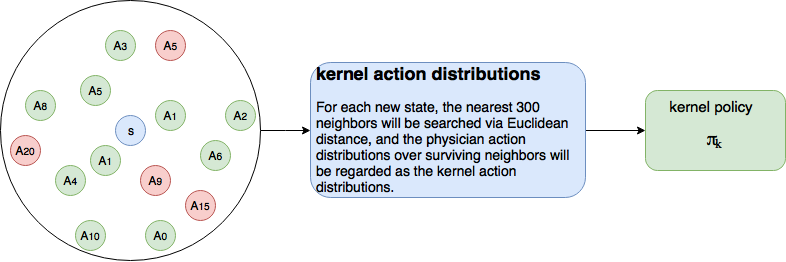
\includegraphics[width=0.55\textwidth]{figures/kernel.png}
\caption{\label{fig:kernel_policy} The circle in the left shows an example of the neighborhoods of a new state $s$, red and green marks the mortality and surviving states respectively, and each of these states is associated with a physician action $A_{i}$.}
\end{figure} 

\textit{DQN Policy.} Double DQN (DDQN) with dueling structure\cite{wang2015dueling}, which is a variant of DQN, has been successfully applied to derive a policy that outperforms the physician policy\cite{DBLP:journals/corr/RaghuKCSG17}. The structure of dueling DDQN is particularly suitable for sepsis treatment strategy learning, as it differentiates the value function $V$ into the value of the patient's underlying physiological condition, called the \textit{Value} stream, and the value of the treatment given, called the \textit{Advantage} stream.  

% FDV: Define those terms, folks won't know what advantage means 

We train the dueling DDQN for 200,000 steps with $batch\,size=32$ to minimize the TD-error. At each given state, the agent is trained to take an action with the highest Q-value, in order to achieve the ultimate goal of improving the overall survival rate.  To stabilize the training process and improve the performance, we applied two techniques: 1) a regularization term $\lambda$ is added to the Q-network loss shown in Equation \ref{eq:qnetwork} to penalize output Q-values which exceed the allowed threshold $r_{max}=3$; to learn the optimal policy more efficiently, 2) prioritized experience replay\cite{schaul2015prioritized}.
\begin{equation}
\label{eq:qnetwork}
\textit{\L}(\theta) = E[(Q_{double-target}-Q(s,a;\theta))^{2}] + \lambda\,\max(|Q(s,a;\theta)-r_{max}|, 0)
\end{equation}
where 
\begin{equation}
Q_{double-target} = r + \gamma Q(s,\argmax_{a^\prime} Q(s,a^\prime;\theta^\prime))
\end{equation}

Finally, given a set of action-values $Q(s,a)$, we must still define a policy $\pi$.  Typically, these actions are chosen by the $\max Q$-value which makes the resulting policy deterministic. Combining a deterministic policy with the stochastic kernel policy to construct the mixture-of-experts is sub-optimal. To avoid this, we took advantage of the dueling double DQN structure to make the DQN policy stochastic. The dueling double DQN estimates the Q-value by approximating the underlying state value (\textit{Value} stream) and the action value (\textit{Advantage} stream) separately.\cite{wang2015dueling} In this way, the \textit{Advantage} stream reflects the qualities of the actions without being affected by the underlying value of the state. Thus, we created a policy action distribution for the DQN expert at each state by applying a \textit{softmax} layer on its \textit{Advantage} stream. 

\section*{Mixture-of-Experts (MoE)}

Due to the heterogeneity of the patient response, it is difficult for one single model to perform well on all types of patients.\cite{parbhoo2017combining} For patient states which are atypical, i.e. farther Euclidean distance away from any neighbors, the kernel expert is unable to generalize resulting in a policy that may be too rigid and conservative. In contrast, DQN experts can over-generalize for these unusual patients. The mixture-of-experts (MoE) combines the kernel and the DQN policies in order to choose the appropriate policy for the appropriate context. The MoE generates mixed policy for any given state based on several characteristics of that state. The Figure \ref{fig:moe} shows the architecture of MoE.


\begin{figure}[H]
\centering
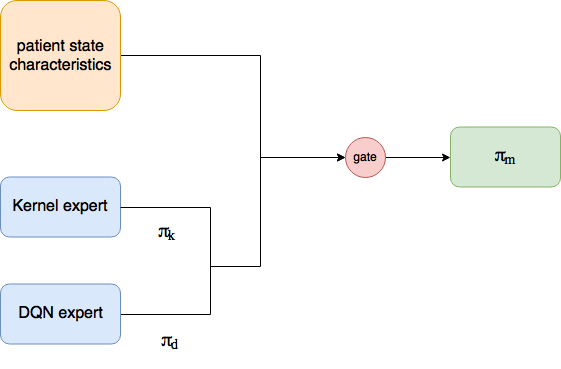
\includegraphics[width=0.45\textwidth]{figures/MOE}
\caption{\label{fig:moe} The architecture of MoE, it produces a mixed policy via combining kernel.}
\end{figure}

\textit{Action Restriction}
In situations where the DDQN has little data, the DDQN can arbitrary policies, including those that suggest actions that were rarely or never performed by clinicians.  To safe guard against actions which may be potentially dangerous, we restricted the actions from the DDQN by the distribution of observed physician actions.  Specifically, we discarded any DDQN suggested action taken less than $1\%$ of the time by the physicians among its 300 nearest neighbors. Let $\pi_{d}(A|S)$ be the DDQN policy, and $\pi_{b}(A|S)$ be the physician policy. The DDQN suggests $\pi_{d}(a|S), a \in A$. If $\pi_{b}(a|S) < 0.01$, then, $\pi_{d}(a|S) \leftarrow 0$. Finally, $\pi_{d}(A|S)$ was normalized to be a valid probability distribution.

We did not restrict kernel policy as it is effectively the physician policy over survivors, and thus cannot deviate too far from clinician actions.  As the MoE policy is a mixture of the kernel and DDQN policy, no additional restriction was needed to safe-guard it.

\textit{Logistic-based Switching}
The primary idea of logistic-based switching is to create a mixed policy per patient per time step that is overall superior to the distinct kernel and DQN policies. A probability as a function of the current state is assigned to each expert. The model used to predict the mortality probability described in \nameref{subsec:rewardformulation} demonstrates the associations between the mortality and various patient demographic and lab values can be found in the \nameref{appendices}. %Appendix~\ref{appendix:gradients}. 
We examined several medical sources \cite{jones2009sequential,beier2011elevation,tamion2010albumin} to determine which features are most useful in the expert selection and chose: age, Elixhauser, SOFA, $FiO_{2}$, BUN, GCS, Albumin, trajectory length, and max distance from neighbors. 

The MoE model's switching function learns the weights and bias for these input features in order to assign probabilities for each expert. The function is described in Equation \ref{eq:moe}, where $X$ denotes the input features, $W_{k}$ and $b_{k}$ denote the weights for the input features and bias in terms of the kernel expert. $p_{k}$ and $p_{d}$ denote the assigned probability for kernel and DQN expert respectively. 

% FDV: Where did the weights and biases come from?  We need to know what function is being parametrized by W,b -> always assume some set of readers will ignore the equations, and the sentences above need to make sense without.

\begin{align}
\label{eq:moe}
\text{sigmoid}(W_{k}X + b_{k}) = p_{k} \\
p_{d} = 1 - p_{k}
\end{align}

\textit{MoE Policy Derivation}
With the expert probabilities assigned for the kernel and DQN experts, the MoE policy is defined as the sum of the products of the expert probabilities and the expert policy action probability distributions. Let $\pi_{k}(A|S)$ and $\pi_{d}(A|S)$ 
respectively denote the probability distribution of actions of the kernel and DQN policies over states. Then, the mixed policy is defined as $\pi_{m}(A|S)=p_{k}\pi_{k}(A|S) + p_{d}\pi_{d}(A|S)$.

%formally in Equation \ref{eq:admoe}.

% \begin{align}
% \label{eq:admoe}
% \pi_{m}(A|S)=p_{k}\pi_{k}(A|S) + p_{d}\pi_{d}(A|S)
% \end{align}

The weights and bias for the input features in the switching function was trained to produce $\pi_{m}(A|S)$ that maximizes the WDR\cite{thomas2016data} estimate of the discounted expected return. The non-concavity of the WDR function makes the optimization challenging, so we conducted a random search of parameters to find local maxima.


\section*{Results}

The estimates of the discounted expected return for each policy are presented in Table \ref{tbl:wdr}.  Both kernel and DQN experts demonstrate an improvement over physician policy. We provide two columns for the mixture of experts policy because it is challenging to derive accurate value estimates $V$ and $Q$ for the WDR estimator in this case (as hard as the original policy evaluation task).  Thus, we consider two sensible options: using the value estimates $V$ and $Q$ from the clinican policy, and using the estimates from the DDQN policy.  Regardless of choice of evaluation covariate, the MoE projects a further improvement. 

% FDV METHOD: You mean you solve for V and Q for the behavior policy rather than the evaluation policy?  Provide more detail here, I'm not sure I follow.  

% XF: solve V and Q for the behavior policy as an approximation for Kernel V and Q.

% FDV: Maybe best as a figure because it is just one line?  And include a way to interpret what these numbers mean w.r.t. mortality 

% XF: maybe table is more space-saving?

\begin{table}[H]
\centering
\caption{Estimate of the discounted expected return for policies over test set, $\gamma=0.99$)} 
\label{tbl:wdr}
\begin{tabular}{|c|c|c|c|c|c|}
\hline
       & Physician & Kernel & DQN  &  $MoE_{V_{b}, Q_{b}}$ & $MoE_{V_{d}, Q_{d}}$ \\ \hline
Estimate & 3.76   & 4.46  & 4.23 & 5.03 & 5.72 \\ \hline
\end{tabular}
\end{table}

\textit{Analysis of discovered policies.}
We present the expert actions in Figure \ref{fig:expert_actions}.  As shown, $a=0$, i.e. no treatment action, is dominant for all policies.  Actions which are in favored by physicians, such as IV but no vasopressor are also prescribed often by the kernel expert. But, our kernel expert tends to be more conservative than the physicians as it suggests no action approximately twice the physicians' frequency--perhaps reflecting a bias toward the fact that those patients who were not treated were somehow healthier and thus survived. In addition, the kernel expert prescribes more fluids when compared with that of physicians. While kernel expert and physician give action high fluids and no vasopressor almost in the same frequency, the kernel expert very rarely suggests actions with vasopressor. Our kernel expert action distribution shares the general behavior of a conservative physician.

The DQN expert, like physicians, favors giving actions a range of fluid values. But, over the test set, DQN expert prescribes more extreme values when compared with physicians. Physicians frequently prescribe high fluids and low vasopressor; however, the DQN expert also tends to give more high vasopressor dosage actions in addition to fluids. 

Over the test set, the behavior of the MoE is much akin to that of the kernel expert, as expected, as most of the states from patients can be mapped into a group of similar states. But driven by the DQN expert, MoE prescribes more high dosage actions. That said, for many given patient states, the actions suggested by experts overlap (see Table \ref{tbl:overlap}). However in 4.4\% of circumstances, the MoE policy follows neither that of kernel nor that of DQN.   

\begin{table}[H]
\centering
\caption{Percent similarity of different policies over test set patient states}
\label{tbl:overlap}
\begin{tabular}{|c|c|c|c|c|}
\hline
           & kernel & DQN   & MoE   \\ \hline
physician  & 0.305  & 0.151 & 0.296 \\ \hline
kernel     & -      & 0.182 & 0.871 \\ \hline
DQN        & -      & -     & 0.258 \\ \hline
\end{tabular}
\end{table}

Finally, to better understand the behaviors of the MoE on forming $\pi_{m}(S|A)$, we show its switching function's parameters $W_{k}$ in Table~\ref{tbl:moe_params}.

\begin{table}[ht]
\centering
\caption{MoE model parameters}
\label{tbl:moe_params}
\begin{tabular}{|c|c|c|c|c|c|c|c|c|c|}
\hline
       & age    & elixhauser & SOFA   & GCS     & FiO2    & BUN     & albumin & traj. len. & max dist.\\ \hline
$W{k}$ & 0.0100 & -0.3328    & 0.0556 & -0.0331 & -0.2714 & -0.3713 & -0.4085 & 0.1429     & -0.4134  \\ \hline
% DQN    & 0.4095 & 0.3261     & 0.2373 & 0.4421  & 0.3600  & 0.4439  & 0.1714  & 0.0149     & -0.1076   & -0.0280 \\ \hline
\end{tabular}
\end{table}

\textit{Evaluation Quality Assessment}
The WDR estimator of policy quality relies on having a large enough collection of patient histories in the evaluation set having non-zero weight $w_t^i$.  For the MoE policy, $90\%$ of the importance sampling weights are non-zero and $86\%$ final weights in the sequences are non-zero. These high numbers of non-zero importance weights indicates that nearly all of our data was used in the evaluation of the policy.  We plot the full distribution of weights in figure \ref{fig:WDR_weights}. A significant number of weights lie in the range of $[10^{-4},10^{-3}]$ and only very few observations have weights significantly larger than that range (the samples with significantly smaller weights are unlikely to have a significant influence on the estimate). However, the few observations with weights on the order of $10^{-1}$ could potentially have large influence.

\begin{figure*}
  \centering
  \begin{subfigure}[b]{0.6\textwidth}
  \centering
  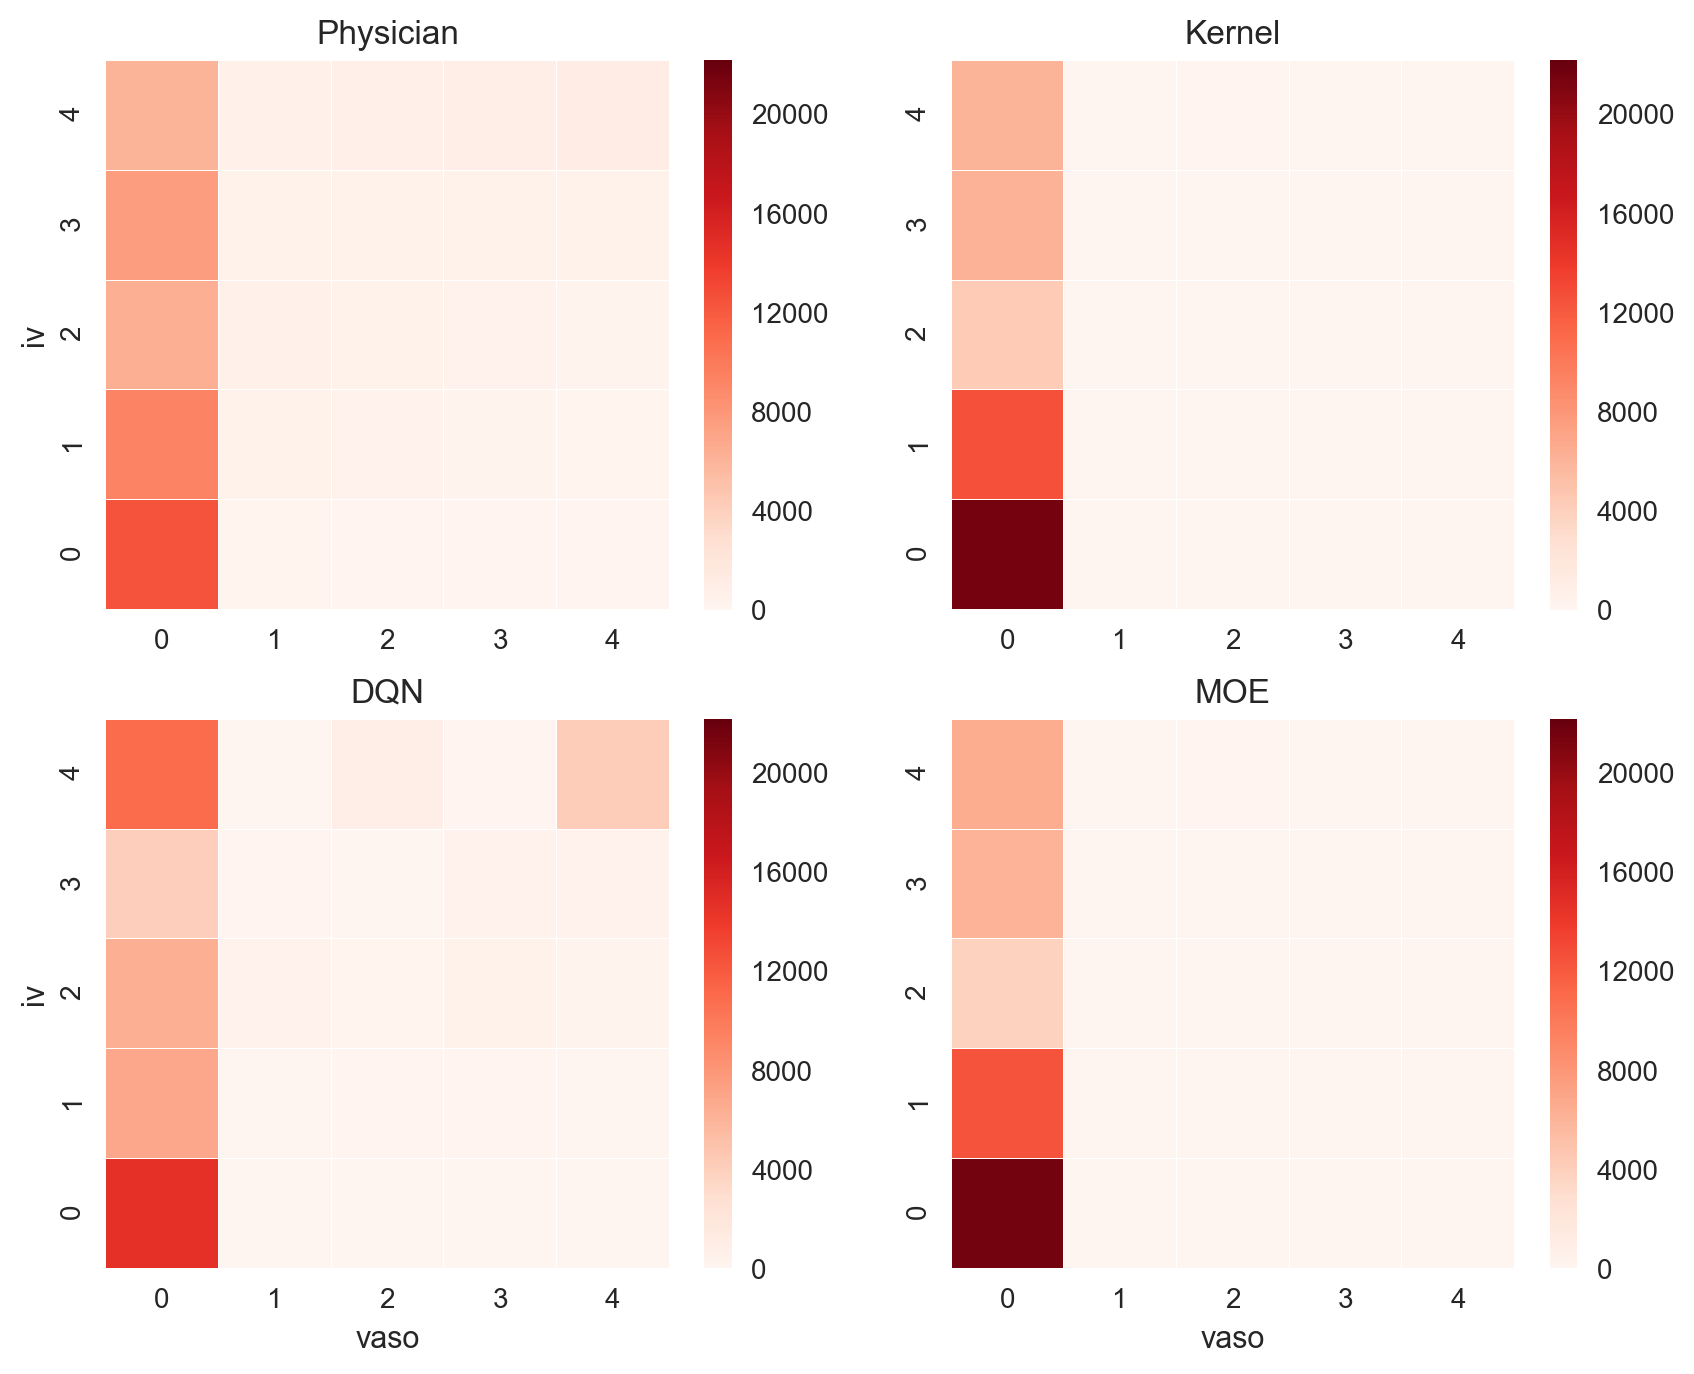
\includegraphics[width=\linewidth]{figures/actions}\hfill
  \caption{\label{fig:expert_actions}Action Distributions for physician and experts over test set}
  \label{fig:twelve:b}
  \end{subfigure}%
  \begin{subfigure}[b]{0.4\textwidth}
  \centering
  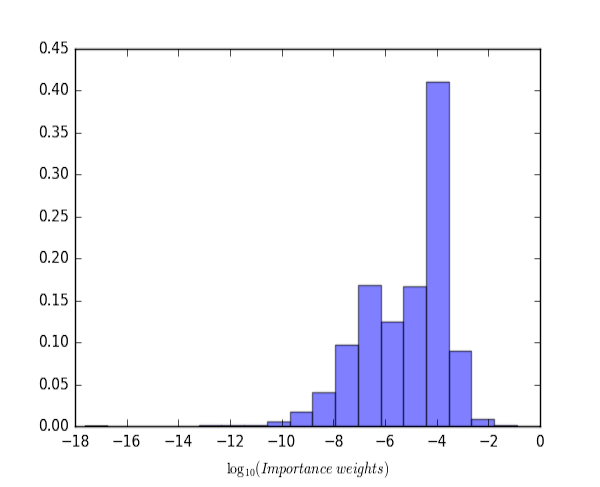
\includegraphics[width=\linewidth]{figures/WDR_weights}\hfill
  \caption{\label{fig:WDR_weights}WDR importance weights distribution}
  \label{fig:twelve:a}
  \end{subfigure}%
  \caption{}
  \label{fig:twelve}
\end{figure*}

% \begin{figure}[H]
% \centering
% 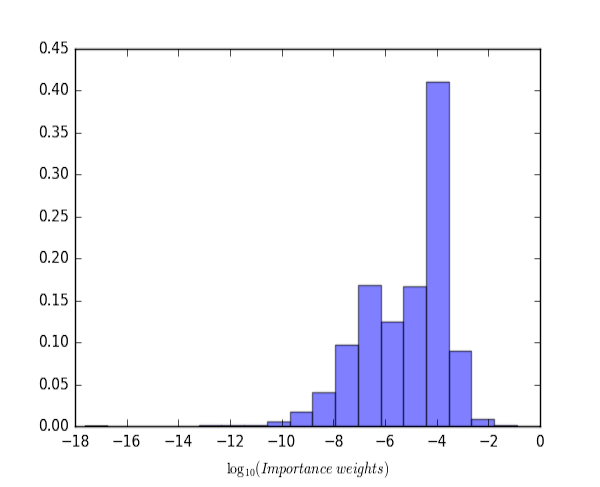
\includegraphics[width=0.5\textwidth]{figures/WDR_weights}
% \caption{\label{fig:WDR_weights} WDR importance weights distribution}
% \end{figure}



% DW: I really don't think we can make this claim - the data does not support it, so I'm commenting it out
%In summary, MoE tends to follow suggestions from kernel expert for patient states with older age, and lower critical lab values except SOFA scores. Furthermore, MoE values kernel more when the given state representation incorporates information from more previous states. With respect to patient states far from from their neighbors, MoE would emphasize DQN expert more. This echoes our assumption that patient far from its neighbors, should be taken care of by the DQN expert.

\section*{Discussion}

A key part of managing sepsis patients is to restore their blood pressure through the administration of intravenous fluids and/or vasopressors. Prescribing an optimal balance between vasopressors and fluids remains challenging. Vasopressors are known to have harmful effects on patients; recent studies have also demonstrated the association between fluid-overload and negative outcomes in the ICUs.\cite{kelm2015}  
Overall, the DQN recommended a treatment strategy with more aggressive use of both vasopressors and fluids.   In comparison to the physician policy, DQN recommended  70\% more actions involving medium-to-high fluid volume and vasopressor dosage (actions 18,19,23, and 24). Most notably, frequency for the DQN action corresponding to maximum levels of both fluid and vasopressor (action 24) increased by 3.8 fold from the physician policy.  These results suggest that while recent advances in deep reinforcement learning aim to learn optimal strategies to guide interventions, further investigations are required, and careful clinical judgment should be exercised to guard against potentially high-risk actions introduced due to instability of non-linear function approximation.   
%physician (actions 18,19,23,24) = 481 + 477 + 898 + 1103 = 2959
%DQN  (actions 18,19,23,24) = 356 + 358 + 126 + 4235 = 5075
%(5075 -2959 ) / 2959 = 0.72

%LL
The proposed kernel expert, in it's current implementation,  recommended far fewer actions involving vasopressors in comparison to both the physician policy and DQN.  While we have chosen to favor a more conservative strategy, e.g. regularizing rare actions as a safety mechanism to guard against unduly aggressive actions,  we recognize that both over and under-treatment can potentially lead to adverse outcomes. Further investigation is required to examine  clinical effects of a conservative kernel expert policy, and whether a more personalized approach may be possible to automatically detect when rare actions are beneficial on an individual patient basis. 
%exploring switching algorithms to improve the balance between the kernel and DQN based approaches.

\textit{Limitations.}
While it appears that our MoE policy significantly outperforms the clinician policy (as well as each individual expert), and we have ensured that the actions it suggests are at least sensible, that is, often taken by clinicians, there still exist a number of limitations.  When encoding the patient clinical course in an LSTM representation, in spite of our high prediction accuracy, we cannot be certain that there are no hidden confounding factors.  Using only survivors in the kernel policy may have biased us toward considering healthier patients, and all optimizations were prone to local optima. 
% FDV: How is this a limitation? 
% In order to reduce DQN instability, we constrained actions to a minimum quorum of physician actions. 

On the evaluation side, the WDR estimator requires either the behavior policy estimate $\pi_b$ to be accurate or the covariate estimates $V$ and $Q$ to be accurate to be unbiased; in our case, we estimated these values to the best of our ability, and showed that our results were at least insenstive to different choices of $V$ and $Q$, but we do not have the true values of either.
% FDV: How is this a limitation?
% Constraining the proposed policies to be close to the clinicians' policies could lead to a narrower distribution of importance weights, and decrease the uncertainty of the method. 

More broadly, our work focused on a very specific subproblem with sepsis management, with a very specific reward structure.  To apply off-policy evaluation (WDR) in a statistically credible way, we considered the accumulation of low mortality risk as the objective, rather than mortality itself (as the latter could not be evaluated reliably).  There also exist many other interventions, such as antibiotics use and mechanical ventilation, that also affect the patient's outcomes.  Finally, our data were limited to the aforementioned fifty variables and only during patients' ICU stays (aside from pre-ICU fluid balance). Future work remains to investigate policies that incorporated a broader scope of patient history as well as a larger variety of interventions.

\section*{Conclusion}

We presented a MoE framework to learn improved fluid and vasopressor administration strategies for sepsis patients in ICUs using observational data.   We demonstrated that the proposed mixture model approach can automatically adapt to patient states at each time step, and dynamically switch between a conservative kernel expert and a more aggressive DQN-generated policy to achieve better expected outcomes than physician, kernel only, and DRL-only experts. While further investigation---such as shadow prospective evaluation---is required to truly validate the efficacy of our approach, the proposed MoE framework represents a novel approach in dynamically switching between two treatment policies, and could potentially provide a safer mechanism to progressively deploy new policies, safe-guarding against actions potentially harmful to the patients. 


%The MoE approach provides a mechanism to automatically switch at each time step between a conservative kernel expert policy and a more aggressive DQN-generated policy. The proposed kernel expert, in it's current implementation,  recommended far fewer actions involving vasopressors in comparison to both the physician policy and DQN.  Further investigation is required to determine if the kernel expert may be overly conservative, and future work will focus on exploring switching algorithms to improve the balance between the kernel and DQN based approaches.  Nevertheless, the proposed MoE framework represents a novel approach in dynamically switching between two treatment policies, and could potentially provide a fail-safe mechanism to progressively deploy new policies, safe-guarding against actions potentially harmful to the patients. 

\section*{Acknowledgments}

We would like to thank the other students in Harvard CS282R - Reinforcement Learning for Healthcare,  Fall 2017 for their insights, encouragement and feedback. Omer Gottesman was supported by the Harvard Data Science Initiative.

\makeatletter
\renewcommand{\@biblabel}[1]{\hfill #1.}
\makeatother



\bibliographystyle{unsrt}
\bibliography{reference}

\begin{appendices}

\section*{Appendices}

\label{appendices}
Due to space constraints, all appendices are available at \\
\href{https://dtak.github.io/cs282-f17-xuefeng-yi-david/peng\_sepsis\_moe\_appendix.pdf}{https://dtak.github.io/cs282-f17-xuefeng-yi-david/peng\_sepsis\_moe\_appendix.pdf}

%--- Appendix A
% \section{Physiological Attributes and Preprocessing}
% \label{appendix:preprocessing}

% The following table summarizes all physiological attributes, treatments and corresponding preprocessing methods
% used in this paper.

% \begin{table}[ht]
% \centering
% %\caption*{Physiological attributes, treatments and corresponding preprocessing methods}
% %\label{table:preprocessing}
% \begin{tabular}{|l|l|}
% \hline
% Preprocessing   & Attributes \\ \hline
% Standardization & \begin{tabular}[c]
% {@{}l@{}}\texttt{age,Weight\_kg,GCS,HR,SysBP,MeanBP,DiaBP,RR,Temp\_C,FiO2\_1,}\\ 
%   \texttt{Potassium,Sodium,Chloride,Glucose,Magnesium,Calcium,Hb,}\\ 
%   \texttt{WBC\_count,Platelets\_count,PTT,PT,Arterial\_pH,paO2,paCO2,}\\ 
%   \texttt{Arterial\_BE,HCO3,Arterial\_lactate,SOFA,SIRS,Shock\_Index,PaO2\_FiO2,}\\ 
%   \texttt{cumulated\_balance\_tev, Elixhauser, Albumin, CO2\_mEqL, Ionised\_Ca}
%   \end{tabular} \\ 
%   \hline
%   Log transformation    & \begin{tabular}[c]
%     {@{}l@{}}\texttt{max\_dose\_vaso,SpO2,BUN,Creatinine,SGOT,SGPT,Total\_bili,}\\
%     \texttt{INR,input\_total\_tev,input\_4hourly\_tev,output\_total,output\_4hourly}
%     \end{tabular}                             \\ \hline
% \end{tabular}
% \end{table}

%--- Appendix C
% \section{Predicted vs True Log-odds Mortality}
% \label{appendix:mortality-log-odds}

% The follow plot shows the predicted vs. true log-odds distribution for survivor and non-survivor classes.
% \begin{figure}[ht]
% \centering
% 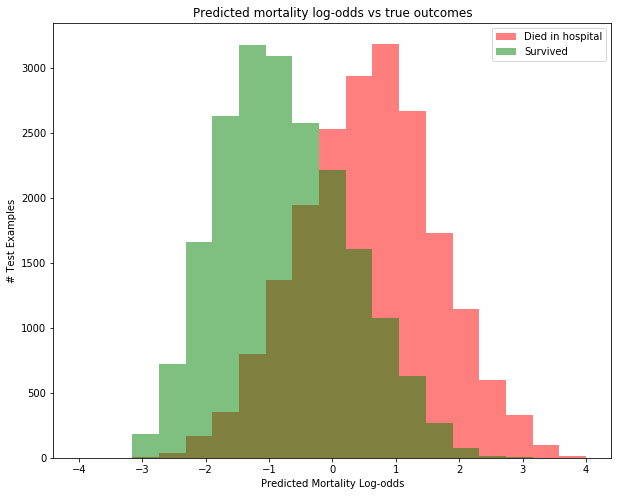
\includegraphics[width=0.7\textwidth]{figures/log-odds.png}
% %\caption{\label{fig:mortality-log-odds} Mortality log-odds distribution for mortality and survivor classes.}
% \end{figure}

%--- Appendix D
% \newpage
% \section{Mortality Gradients vs. Feature Values}
% \label{appendix:gradients}

% The following set of plots shows mortality gradients versus feature values. No single observation value is highly correlated with mortality.

% \begin{figure}[ht]
% \centering
% 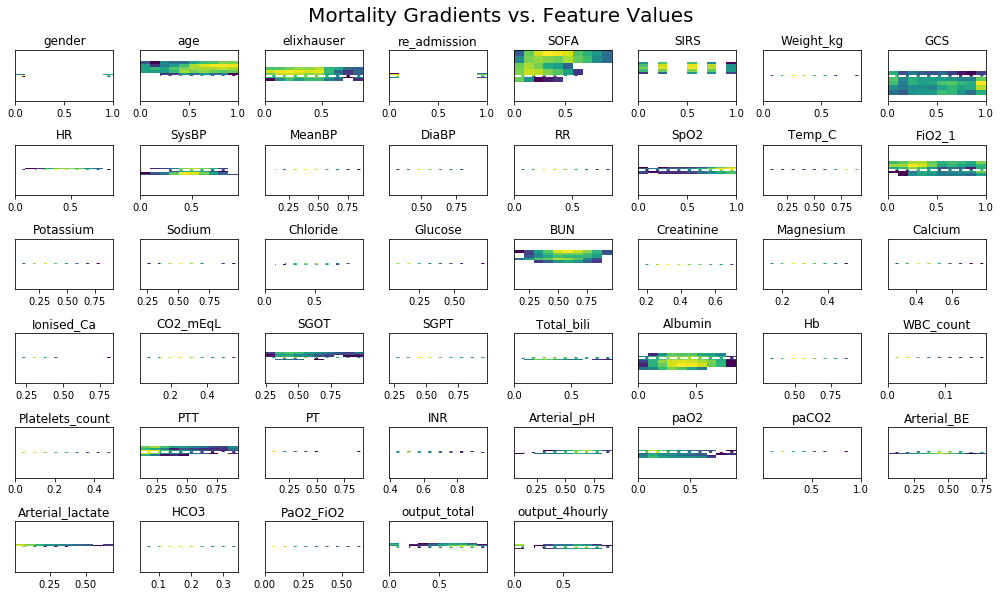
\includegraphics[width=0.9\textwidth]{figures/gradients}
% %\caption{\label{fig:gradients} Mortality gradients versus feature values. No single observation value is highly correlated with mortality.}
% \end{figure}

\end{appendices}


\end{document}







